\documentclass{article}
\usepackage[utf8]{inputenc}
\usepackage{amsmath,amsthm,amssymb}
\usepackage[unicode,colorlinks=true,citecolor=green!40!black,linkcolor=red!20!black,urlcolor=blue!40!black,filecolor=cyan!30!black]{hyperref}
\usepackage{tikz}
\usetikzlibrary{calc}
\usetikzlibrary{decorations.shapes, shapes.geometric}

\begin{document}

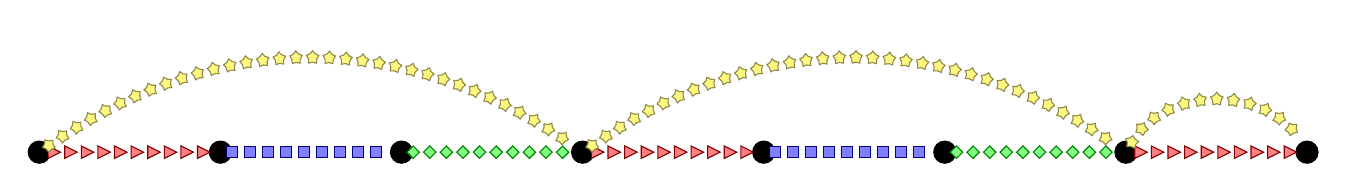
\begin{tikzpicture}[scale=2.3]
 \tikzstyle{vertex}=[draw,circle,fill,minimum size=8,inner sep=0]
 \tikzset{paint/.style={draw=#1!50!black, fill=#1!50}, decorate with/.style = {decorate, decoration={shape backgrounds, shape=#1, shape size = 4.5pt, shape sep = 6pt}}}
 \tikzstyle{edge_red}=[draw, decorate with = isosceles triangle, paint = red]
 \tikzstyle{edge_blue}=[draw, decorate with = rectangle, decoration = {shape size = 4pt, shape sep = 6.5pt}, paint = blue]
 \tikzstyle{edge_green}=[draw, decorate with = diamond, paint = green]
 \tikzstyle{edge_yellow}=[draw, decorate with = star, paint = yellow]
 
 \node[vertex] (a1) at (1,0) {};
 \node[vertex] (a2) at (2,0) {};
 \node[vertex] (a3) at (3,0) {};
 \node[vertex] (a4) at (4,0) {};
 \node[vertex] (a5) at (5,0) {};
 \node[vertex] (a6) at (6,0) {};
 \node[vertex] (a7) at (7,0) {};
 \node[vertex] (a8) at (8,0) {};
 
 \draw[edge_red] (a1) -- (a2);
 \draw[edge_red] (a4) -- (a5);
 \draw[edge_red] (a7) -- (a8);
 
 \draw[edge_blue] (a2) -- (a3);
 \draw[edge_blue] (a5) -- (a6);
 
 \draw[edge_green] (a3) -- (a4);
 \draw[edge_green] (a6) -- (a7);
 
 \draw[edge_yellow, bend left=35] (a1) to (a4);
 \draw[edge_yellow, bend left=35] (a4) to (a7);
 \draw[edge_yellow, bend left=60] (a7) to (a8);
\end{tikzpicture}

\end{document}